%%!TEX TS-program = latex
\documentclass[]{beamer}
%\usepackage{helvet}
%\usepackage{pstricks,pst-node,pst-tree}
\usepackage{graphicx}
\hypersetup{pdfpagemode=FullScreen}
\usetheme{Singapore}
%\usetheme{copenhagen}
%\usetheme{Boadilla}
%\usetheme{Warsaw} 
\usecolortheme{seagull} 
\setbeamercovered{transparent}
\beamertemplatenavigationsymbolsempty 
\setbeamertemplate{footline}[frame number]

\usepackage{hyperref}
\usepackage{amsmath}
\usepackage{amsfonts}
\usepackage{amssymb}
\usepackage{dsfont}

\newcommand{\R}{\ensuremath{\mathds{R}}}
\newcommand{\C}{\ensuremath{\mathds{C}}}
\newcommand{\Q}{\ensuremath{\mathds{Q}}}
\newcommand{\N}{\ensuremath{\mathcal{N}}}
\newcommand{\Z}{\ensuremath{\mathds{Z}}}

\setbeamerfont{bib}{size*={4.00}{4.00}}
\usepackage[square, sort, numbers, authoryear]{natbib}
\renewcommand{\bibsection}{\subsubsection*{\bibname } }


\DeclareMathOperator*{\argmax}{argmax}
\DeclareMathOperator*{\Corr}{Corr}
\DeclareMathOperator*{\E}{E}
\DeclareMathOperator*{\sign}{sign}
\renewcommand{\vec}[1]{\mathbf{#1}}
\usepackage{hyperref}

\usepackage{multicol}
\usepackage{multirow}
\usepackage{pbox}


\institute[]{}
%\logo{\pgfimage[width=.8cm,height=.8cm]{../KU_logo}}
\title[]{
{
Predicting political party affiliation from text
}}
\author{
Felix Biessmann\thanks{~\tt felix.biessmann@gmail.com}\\
 Pola Lehmann\thanks{ ~{\tt pola.lehmann@wzb.eu} }\\
%  WZB f\"ur Sozialforschung\\
Daniel Kirsch\\
  Sebastian Schelter\thanks{~\tt sebastian.schelter@tu-berlin.de}\\
}

\begin{document}

\begin{frame} 
\titlepage 
\end{frame}	

%
%\section{Intro}
%\subsection{}

\begin{frame}\frametitle{Disclaimers}
\small
\begin{itemize}[<+->]
\item (For me) This is just a hobby -- it has nothing to do with my job
\item I did not know a lot of literature in the field 
%\begin{itemize}
\item Some of this might sound naive (like the title)
%\item I hope nobody (who has been active in the field for years) takes this personal
%\end{itemize}
\end{itemize}
\end{frame}

%\begin{frame}\frametitle{Motivation}
%\begin{itemize}[<+->]
%\item Media generate
%\end{itemize}
%\end{frame}

%\begin{frame}\frametitle{Overview}
%\small
%\begin{itemize}[<+->]
%\item Methods 
%\begin{itemize}
%\item Data
%\item Preprocessing
%\item Classification Model
%\end{itemize}
%\item Results
%\begin{itemize}
%\item In-domain held-out data
%\item Out-of-domain held-out-data
%\end{itemize}
%\item Challenges of automated analyses
%\item Tools for better interpretability / leveraging domain knowledge
%\item Conclusion
%\item Web applications of political bias prediction
%\end{itemize}
%\end{frame}

\section{Methods}
\subsection{}

\begin{frame}\frametitle{Data}
\begin{itemize}
\item In-domain data (training data domain)
\begin{itemize}
\item \url{http://www.bundestag.de/plenarprotokolle}
\end{itemize}
\vspace{1em}
\item Out-of-domain data (test data domain)
\begin{itemize}
\item \url{https://manifestoproject.wzb.eu/}
\item Texts from public Facebook pages of parties
\end{itemize}
\end{itemize}
\end{frame}

\begin{frame}\frametitle{Preprocessing}
\begin{itemize}
\item Basic text cleaning (regexps, stopwords)
\item Stemming
\item n-grams (1-5)
\item Tf-idf normalisation
\end{itemize}
\end{frame}

\begin{frame}\frametitle{Classification Model: Multinomial Logistic Regression}
Party affiliation estimate is modelled as
\begin{eqnarray}\label{eq:logreg_multiclass}
p(y=k|\vec{x}) = \frac{e^{z_k}}{\sum_{j=1}^K e^{z_j}}  \textrm{ with }  z_k=\vec{w}_k^{\top}\vec{x}.
\end{eqnarray}
With
\begin{itemize}
\item Labels $y\in\{1,2,\dots,K\}$ (true party affiliation)\\ 
\item $\vec{w}_1,\dots,\vec{w}_K\in\R^{d}$ weight vectors of $k$th party\\ 
\end{itemize}
\end{frame}

\begin{frame}\frametitle{Model Selection}
\begin{block}{}
\centering
All hyperparameters optimised with nested cross-validation.
\end{block}
\end{frame}

\section{Results}
\subsection{}


\begin{frame}\frametitle{Results: In-domain Predictions}

\begin{table}[t]
\caption{
\label{tab:results_in-domain}
{\bf 17th Bundestag}}
\begin{center}
\begin{tabular}{lcccc}
    &         precision    &recall &  f1-score  & N  \\
\hline \hline
       cducsu   &    0.62  &    0.81  &    0.70  &     706\\
        fdp    &   0.70   &   0.37  &    0.49    &   331\\
     gruene &      0.59  &    0.40   &   0.48   &    298\\
      linke    &   0.71   &   0.61  &    0.65    &   338\\
        spd   &    0.60   &   0.69  &    0.65   &    606\\
\hline
 total &      0.64   &   0.63   &   0.62    &  2279 
%
\end{tabular}
\end{center}
\end{table}

\end{frame}


\begin{frame}\frametitle{Results: Out-of-domain Predictions}

\begin{table}[t]
\caption{
\label{tab:results_out-of-domain}
{\bf Tested on manifesto quasi-sentences}}
\begin{center}
\begin{tabular}{lcccc}
    &         prec.    &recall &  f1-score  & N  \\
\hline \hline
    cducsu    &   0.26   &   0.58   &   0.36    &   2030 \\
    fdp    &   0.38   &   0.28   &   0.33    &   2319 \\
     gruene   &    0.47    &  0.20   &   0.28    &  3747\\
      linke     &  0.30  &    0.47    &  0.37    &   1701\\
        spd     &  0.26  &    0.16   &   0.20    &   2278\\
\hline
total    &   0.35  &    0.31  &    0.30   &   12075\\
%
\end{tabular}
\end{center}

\end{table}

\end{frame}

\section{Challenges}
\subsection{}

\begin{frame}\frametitle{Why is out-of-domain classification so bad?}
\begin{enumerate}
\item Length of texts
\vspace{2em}
\item Text domain differences
\end{enumerate}
\end{frame}

\begin{frame}{Effect of Text Length}
\only<1>{
\begin{table}[t]
\caption{
\label{tab:results_topic}
(topic level) {\bf Manifesto data predictions}}
\begin{center}
\begin{tabular}{lcccc}
    &         precision    &recall &  f1-score  & N  \\
    \hline
        \hline
cducsu     &  0.64  &    1.00  &    0.78    &     7\\
       fdp    &   1.00    &  1.00    &  1.00    &     7\\
    gruene  &     1.00  &    0.86  &    0.92    &     7\\
     linke    &   1.00   &   1.00     & 1.00    &     7\\
       spd   &    0.80   &   0.50    &  0.62     &    8\\
    \hline
total  &     0.88   &   0.86   &   0.86  &      36\\
\end{tabular}
\end{center}
\end{table}
}
\only<2>{
\begin{table}[t]
\caption{
\label{tab:results_fb}
 {\bf Facebook post predictions} (text length: 1000 words).}
\begin{center}
\begin{tabular}{lcccc}
    &         precision    &recall &  f1-score  & N  \\
    \hline
        \hline
 cducsu     &  0.65     & 1.00  &    0.79     &   50\\
     gruene   &    0.67   &   0.12  &    0.20   &     50\\
      linke       &0.60    &  0.82    &  0.69    &    50\\
        spd       &1.00 &     0.92   &   0.96    &    50\\
\hline
avg / total    &   0.73   &   0.71  &    0.66   &    200\\
\end{tabular}
\end{center}
\end{table}
}
\only<3>{
\begin{itemize}
\item Longer texts are easier to predict
\item Intuitively makes sense
\item In line with previous findings, see e.g. \cite{Hirst2014}
\item But still, accuracies are far from perfect
\end{itemize}
}
\only<4>{
\centering
What -- except length -- decreases generalization performance? 
}
\end{frame}

\begin{frame}{Effect of Text Domain}
\centering
\only<1>{
\begin{table}[t]
\caption{
\label{tab:results_binary_17}
Classification texts into government and opposition (long texts).
}
\begin{tabular}{lccc}
& {\bf In-Domain} & \multicolumn{2}{c}{{\bf Out-of-Domain}}\\
& Parliament & Manifestos & Facebook Posts\\
\hline
Accuracy    &   0.88   &   0.60&      0.76\\
%
\end{tabular}
\end{table}

\begin{itemize}
\item Despite less noisy, longer texts:\\
{\bf Accuracy on manifesto data close to chance}
\end{itemize}
}
\only<2>{
\begin{itemize}
\item Recognized in previous work, see e.g. \cite{Yu2008}
\item Every ML model is biased by its training data
%\item Political scientists have less of a problem with varying domains
\item Generalization from biased data is {\em the} central problem of ML
\item Strategies to improve generalization
\begin{itemize}
\item Empirical risk minimization / Regularization
\item More (heterogeneous) data
\item Better models: \\ Cov. shift adaptation, transfer/semi-supervised learning,  \dots
\item {\bf Domain knowledge}
\end{itemize}
\vspace{1em}
\item[$\rightarrow$] 
\centering
How can political scientists leverage domain knowledge for automatic text analysis models?
\end{itemize}
}
\end{frame}

\section{Tools}
\subsection{}

\begin{frame}{Some ML Tools for Leveraging Domain Knowledge}
\begin{itemize}
\item Relation between misclassifications and party policy
\item Covariation Text Features and Party labels \\({\bf not model coefficients!}) \cite{Haufe2013}
\item Explicit tests of domain knowledge: Sentiment and Power
\end{itemize}
\end{frame}

\begin{frame}{Sentiment correlates with political power}
\begin{center}
\only<1>{
17th Bundestag\\
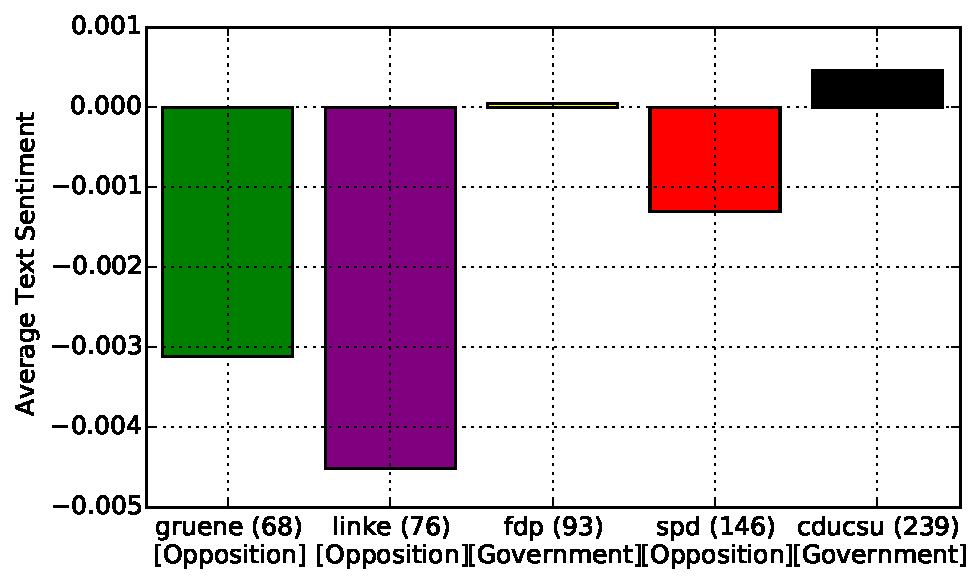
\includegraphics[width=0.7\textwidth]{images/party-sentiments-17}\\
}
\only<2>{
18th Bundestag\\
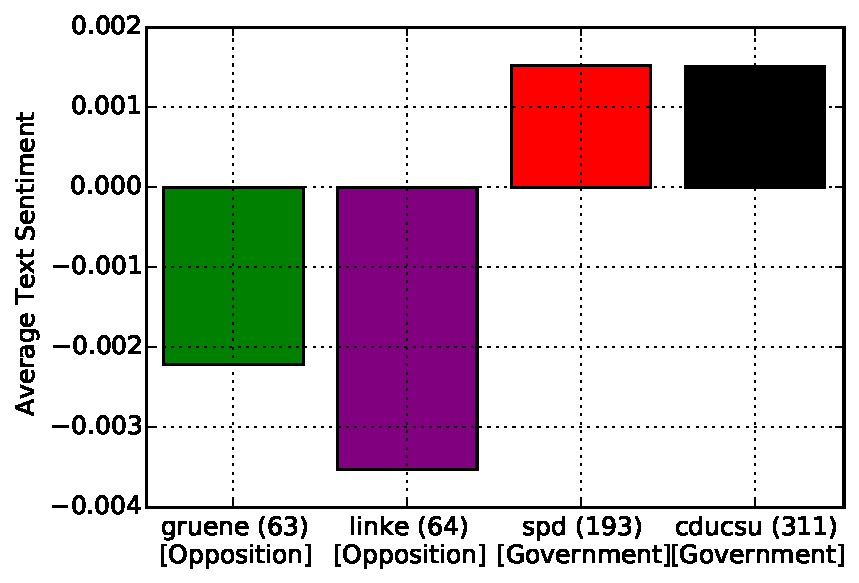
\includegraphics[width=0.7\textwidth]{images/party-sentiments-18}\\
}
\only<3>{
\begin{table}[t]
\caption{
\label{tab:sentiments}
\centering
Correlation coefficient between average sentiment with government membership and number of seats in the parliament.
}
\begin{tabular}{lcc}
   Sentiment vs. &          Gov. Member    &  Seats\\
\hline\hline
17th Bundestag    &  0.84 & 0.70\\
18th Bundestag   &  0.98 & 0.89\\
%
\end{tabular}
\end{table}
}
\end{center}
\end{frame}

\begin{frame}\frametitle{Finding Discriminative Features}
\centering
\only<1>{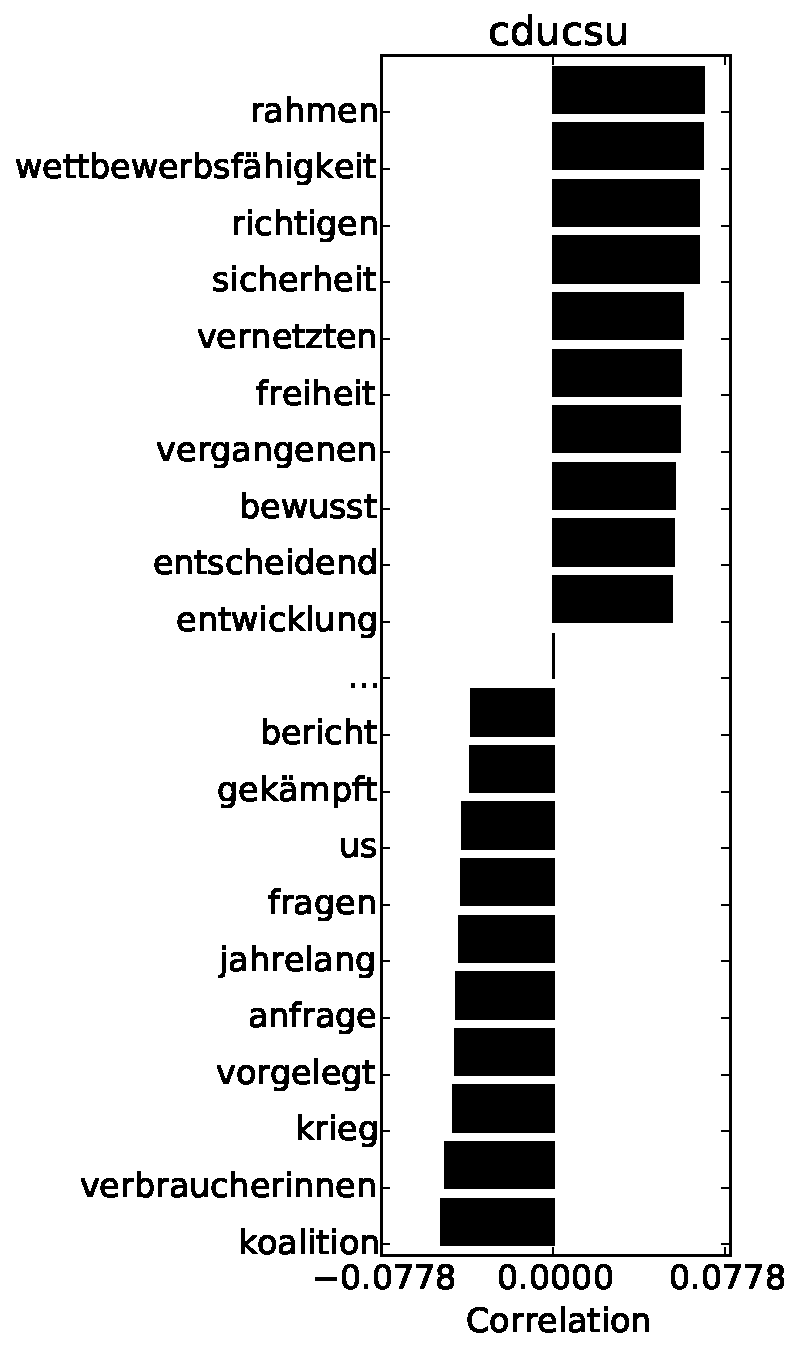
\includegraphics[width=0.4\textwidth]{images/party_word_correlations-cducsu-18}}
\only<2>{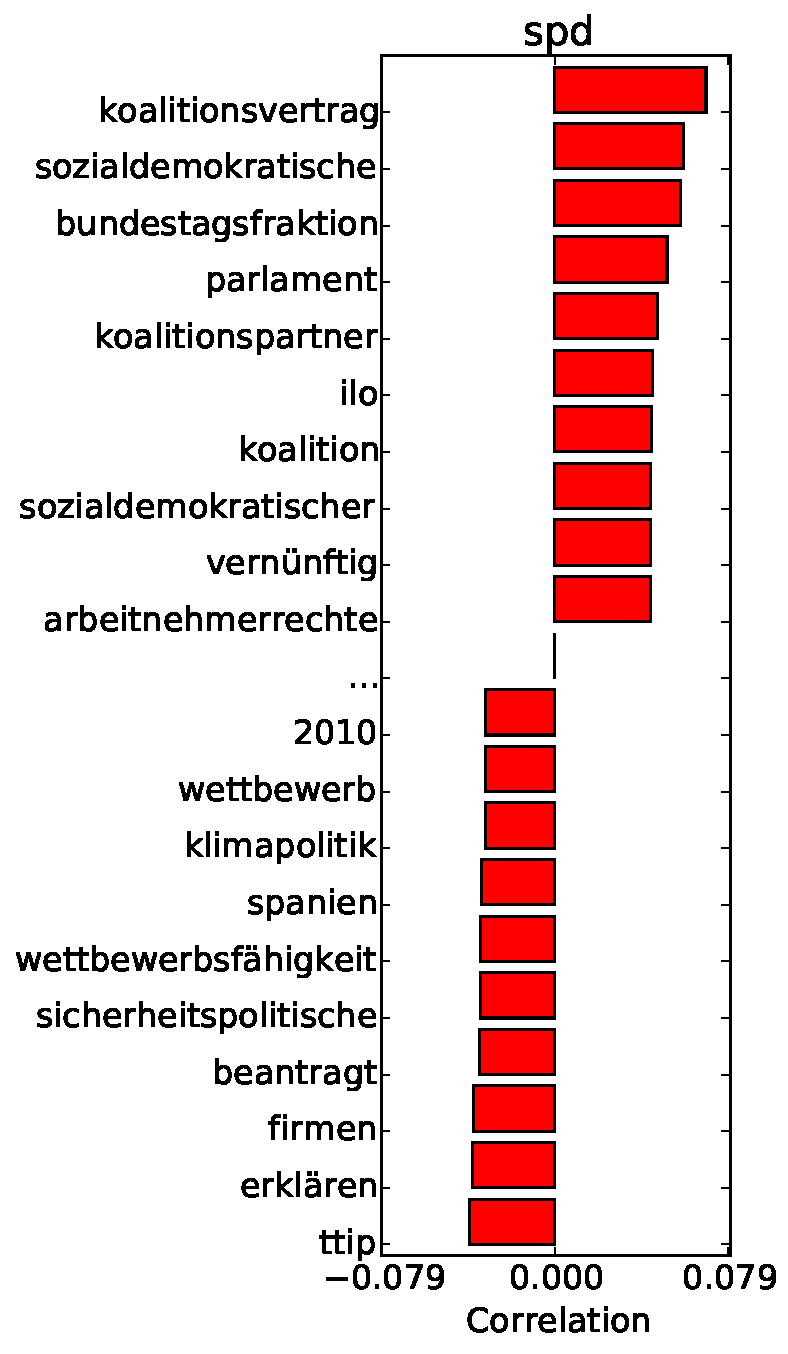
\includegraphics[width=0.4\textwidth]{images/party_word_correlations-spd-18}}
\only<3>{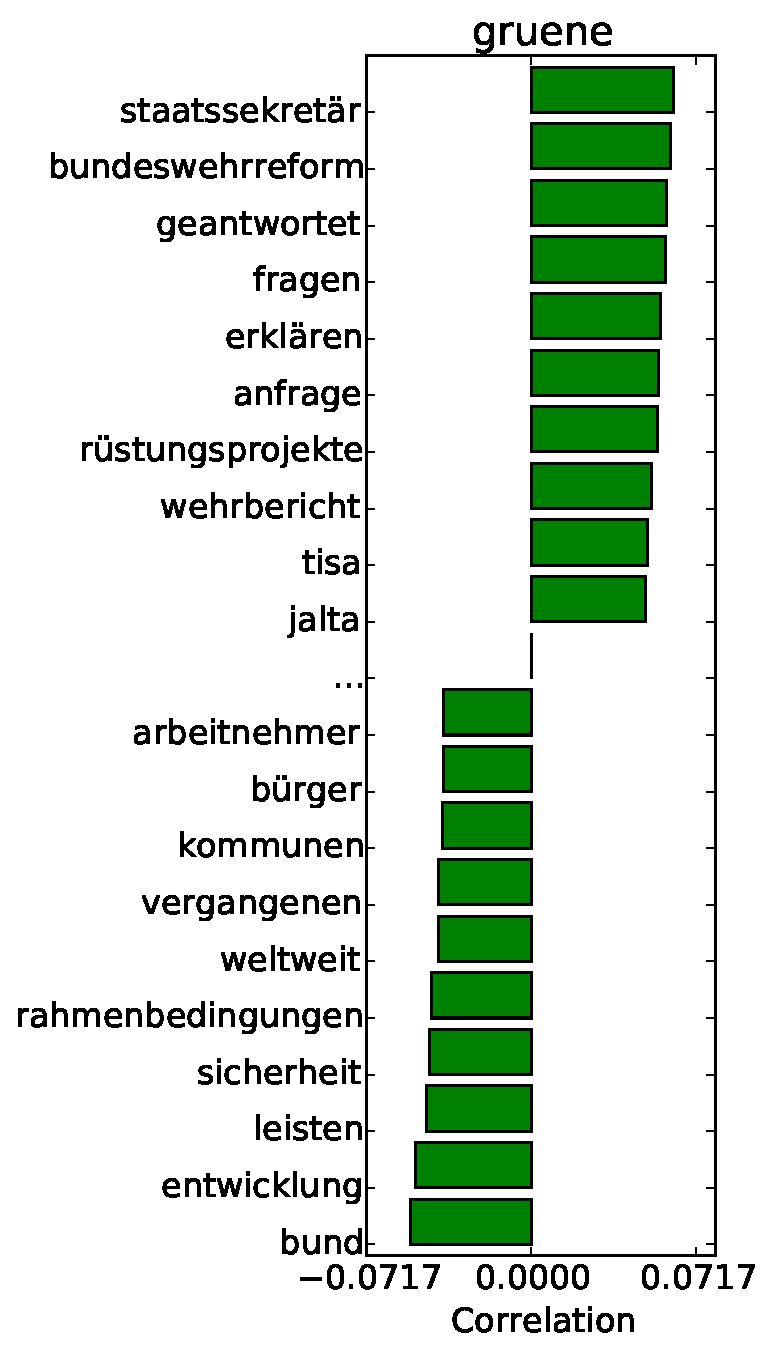
\includegraphics[width=0.4\textwidth]{images/party_word_correlations-gruene-18}}
\only<4>{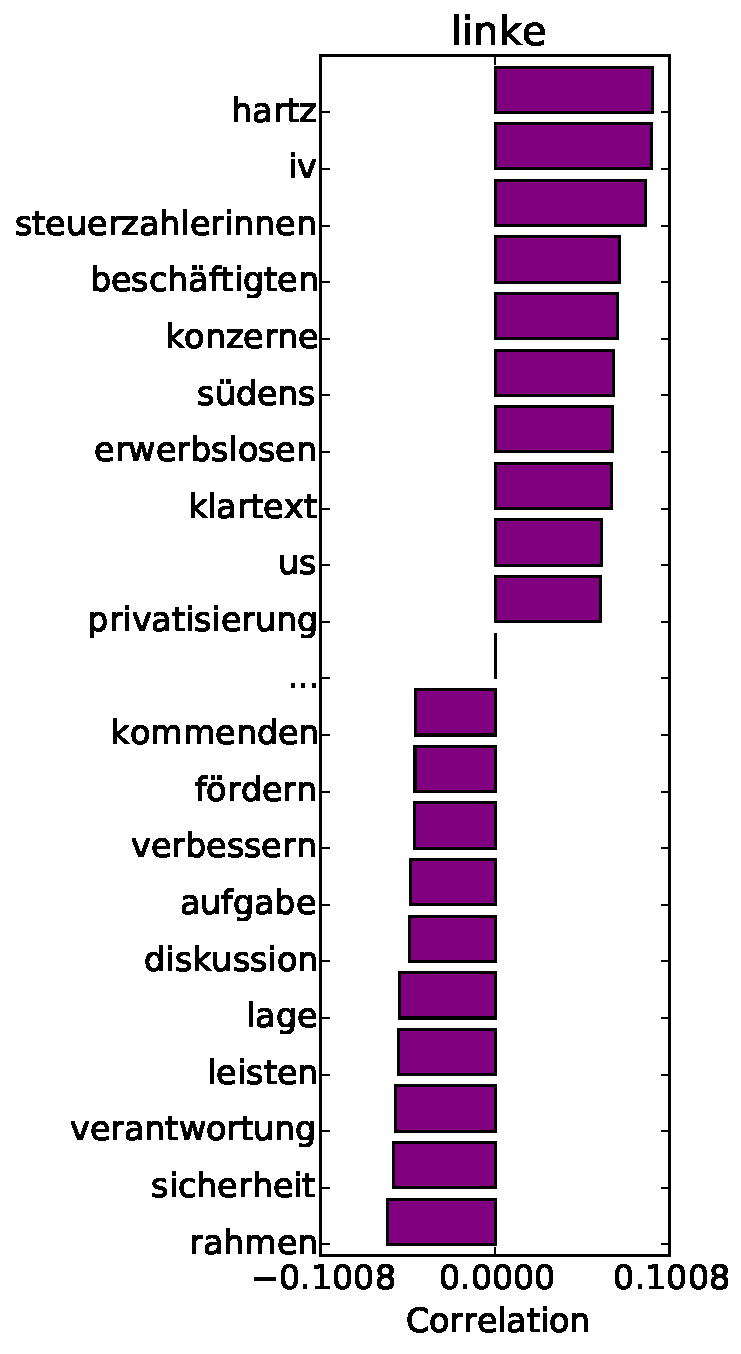
\includegraphics[width=0.4\textwidth]{images/party_word_correlations-linke-18}}
\end{frame}

\begin{frame}\frametitle{Misclassifications and Policy Change}
\centering
Confusion Matrix 17th Bundestag\\
\vspace{1em}
\begin{tabular}{lc|ccccc}
&& \multicolumn{5}{c}{\bf Predicted}\\
&& cducsu & fdp& gruene& linke& spd\\
\hline
\multirow{5}{*}{\rotatebox{90}{\pbox{2cm}{\centering {\bf True}}}} &cducsu &7& 0& 0& 0& 0\\
&fdp&0& 7& 0& 0& 0\\
&gruene&0& 0& 6& 0& 1\\
&linke&0& 0& 0& 7& 0\\
&spd&4& 0& 0& 0& 4\\
\end{tabular}
\end{frame}

\section{Conclusion}
\subsection{}


\begin{frame}\frametitle{Conclusion}
\begin{itemize}
\item Out-of-domain prediction of political bias possible
\item Challenges
\begin{itemize}
\item Text length, see also \cite{Hirst2014}
\item Domain transfer, see also \cite{Hirst2014, Yu2008}
\end{itemize}
\item Generalization should leverage domain knowledge
\item Tools for leveraging domain knowledge
\begin{itemize}
\item Relating misclassifications to policy changes
\item Interpreting discriminative features
\item Testing human experts' hypotheses explicitly
\end{itemize}
\end{itemize}
\end{frame}

\begin{frame}\frametitle{Some Web Applications}
\centering
\only<1>{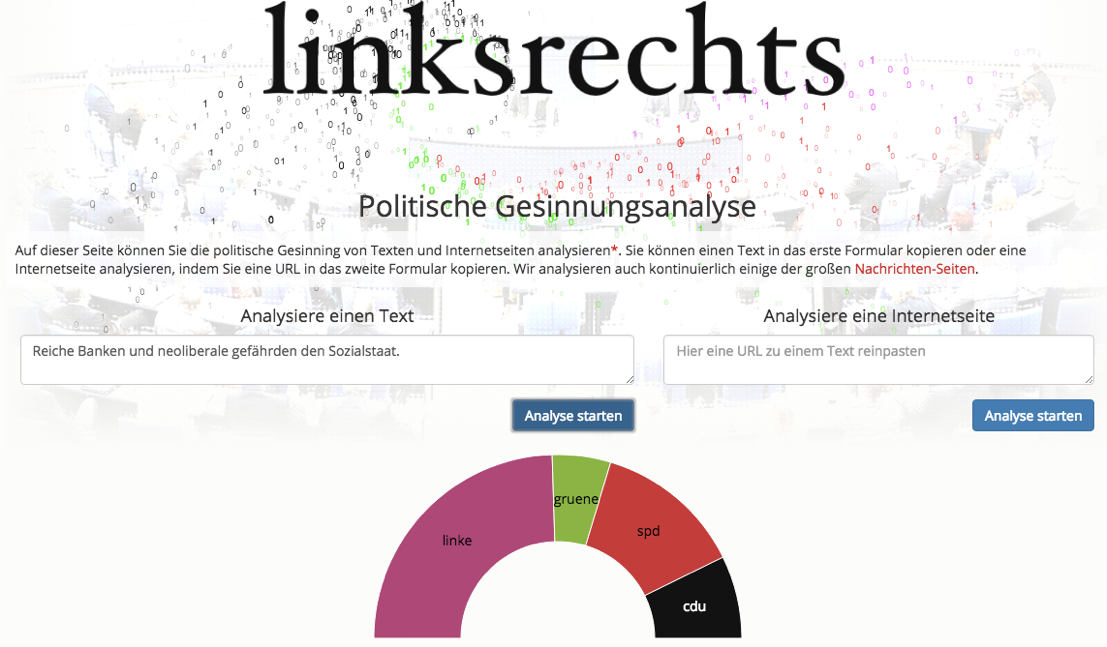
\includegraphics[width=0.7\textwidth]{images/linksrechts-screenshot-1}}
\only<2>{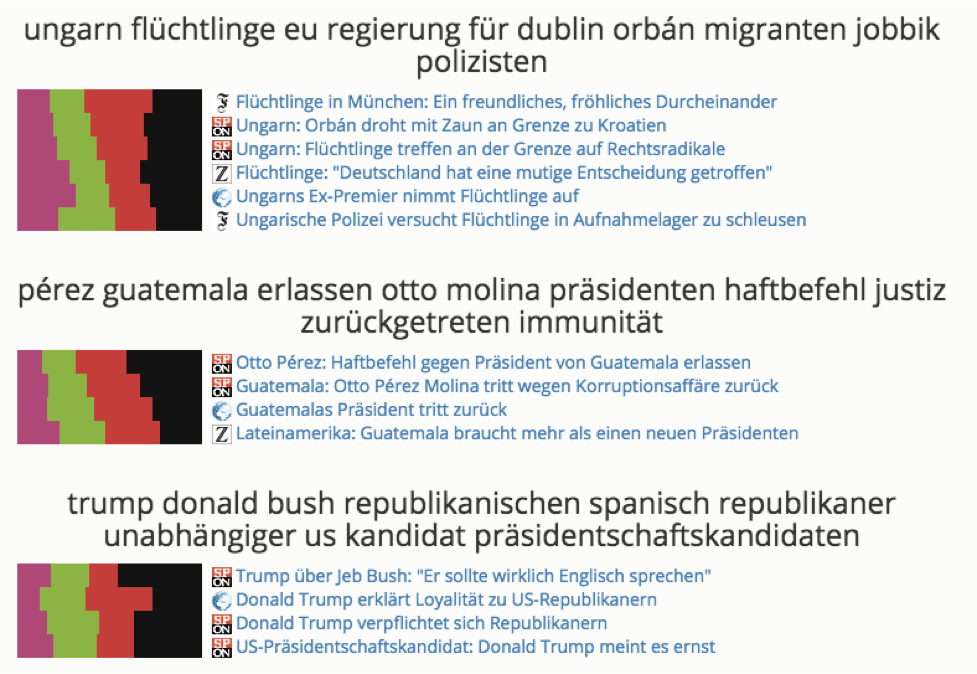
\includegraphics[width=0.7\textwidth]{images/linksrechts-screenshot-2}}
\only<3>{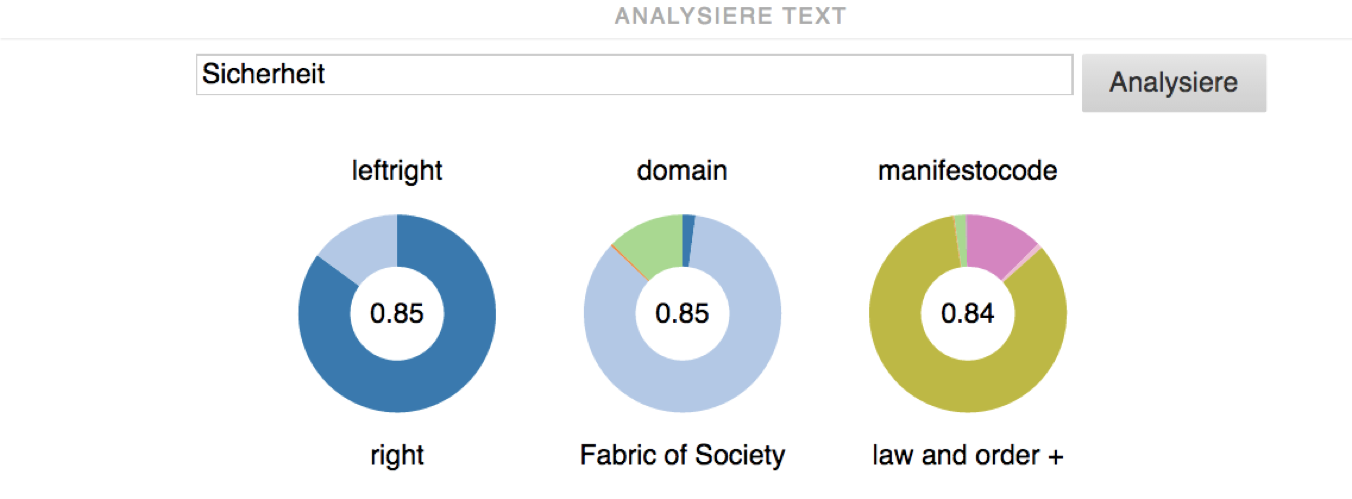
\includegraphics[width=0.7\textwidth]{images/fipi-screenshot-2}}
\only<4->{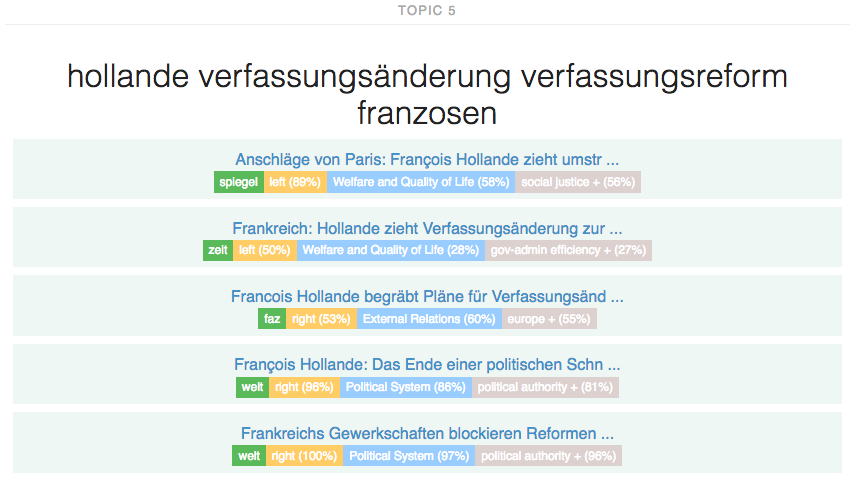
\includegraphics[width=0.7\textwidth]{images/fipi-screenshot}}
\end{frame}

\begin{frame}\frametitle{PyData Hackathon 2016 Berlin}
\centering
\begin{minipage}{0.3\textwidth}

\includegraphics[width=.6\textwidth]{images/pydata-logo-berlin-2016}\\
\end{minipage}
\begin{minipage}{0.6\textwidth}
\small
\begin{itemize}
\item[What?] Follow-up event of PyData Berlin 2016\\
\item[] Inviting Data Scientists, Social Scientists, UX Designers, \dots
\item[] Data Ambassadors for 
\begin{enumerate}
\item Manifesto Data
\item Parliament Data
\item Social Network Data
\end{enumerate}
\item[When?] First weekend of October 2016 (1.-2.)
\item[Where?] Berlin 
\end{itemize}
\end{minipage}
\end{frame}
%
%
\begin{frame}\frametitle{References}
\usebeamerfont{bib}

\bibliographystyle{abbrvnat}
\def\newblock{}
\vspace{2em}
\bibliography{political_bias_prediction} 
\end{frame}

\end{document} 
